\input preamble.tex
\noindent
\section*{Industrielektronikk Øving 02 - Bryter og LED (lys) }

I denne øvingen skal du bruke koblingsbrettet til å koble sammen en bryter og en type lys kalt LED. Dette er en vanlig type kobling i styre kretser. En bryter styrer spenningen til en belastning, i denne øvingen et lyd av typen LED. \\

LED står for Light Emitting Diode og er etterhvert blitt en vanlig type lys. Når en kjøper en LED til å ha i huset koblet denne i lampesokkelen, og en ternger ikke tenke mer over det. En LED er egetlig avhengig av at strømmen går rett vei igjennom. Du må være nøye med at strømmen går med pilen som LED-en er merket med
\noindent \begin{center}
\begin{figure}[H]
\noindent \begin{centering}
%\includegraphics[angle=90,width=16cm]{\string"tegninger/Elektroteknikk - Breadboard\string".pdf}\vspace{2cm}
\par\end{centering}
\noindent \begin{centering}
%\includegraphics[width=16cm]{\string"tegninger/Elektroteknikk - koblingsbrett\string".jpg}
\par\end{centering}
$$\includegraphics[width=10cm]{./lIndustrielektronikk02.eps}$$
\end{figure}
\par\end{center}

\subsubsection*{Utstyr du trenger}
\begin{itemize}
\item Labbrettet
\item Rød og svart isolert ledning
\item LED 
\item Bryter
\item Multimeter
\end{itemize}

\subsubsection*{Oppgaven}
Koble bryteren og LED i serie. Det er vanlig å sette bryteren nærmest +24V tilkoblingen
\begin{enumerate}
		
		\item Trykk inn bryteren, lyster LED-en?
		\item Mål spenningen over LED-en 
		\item Koble et ampermeter i serie med LED-en og mål strømmen igjennom LED-en
\end{enumerate}

\subsubsection*{Innlevering}

Skriv en labrapport og lever på OneNote
\underbar{file ./lIndustrielektronikk01.tex}
\vskip 5pt 

\end{document}

